% !TEX program  = xelatex
% pdflatex.exe -synctex=1 -interaction=nonstopmode -shell-escape %.tex
\documentclass{article}
\usepackage[ruled,vlined,linesnumbered]{algorithm2e}
\usepackage{newtxtext}
\usepackage{algpseudocode}
\usepackage{amsmath}
\usepackage{amsthm}
\usepackage{graphicx}
\usepackage{subfigure}
\usepackage{float}
\usepackage{amsmath }
\usepackage{amsfonts }
\usepackage{pdfpages}
\usepackage{epsfig}
\usepackage{graphicx}
\usepackage{arydshln}
\usepackage{verbatim}
\usepackage{subfigure}
\usepackage{enumerate}
\usepackage{rotating}
\usepackage{threeparttable}
\usepackage{caption}
\usepackage{tikz}
\usepackage{epsfig}
\usepackage{cite}
\usepackage{geometry}
\usepackage{fontspec}
\setmainfont{Times New Roman}
\geometry{a4paper, top=2.4cm, bottom=2.4cm, left=3cm, right=3cm}
\theoremstyle{definition}
\newtheorem{prob}{Problem}
\newtheorem{ans}{Answer}
\usepackage[colorlinks,linkcolor=black]{hyperref}
\linespread{1}
\usepackage{minted}
\begin{document}
	\title{AI3604 Computer Vision}
	\author{Kailing Wang 521030910356}
	\date{September 28.2023}
	\maketitle
	\section*{Written Assignment}
%	\begin{enumerate}[1)]
%		\item Consider a pinhole camera with perspective projection.
%		\begin{enumerate}[a.]
%			\item (10 points) Consider a circular disk that lies in a plane parallel to the image plane. The disk does not necessarily lie on the optical axis. What is the shape of the image of the disk? Show your work and derive your equations.
%			\item (10 points) In class, we discussed how to find the vanishing point of lines. 
%			
%			Suppose I now consider a family of lines that all lie in a single plane. Where on	the image would the vanishing points of \textbf{ALL} lines on the plane $A x+B y+C z+D=$ 0 lie? The coordinate frame is located at the pinhole with the z-axis pointing towards the image and the effective focal length is $\boldsymbol{f}$.
%			
%			First, start with a simple case where $A=C=D=0$ and $B=1$ which defines a plane extending horizontally from the optical center. Write down three different line directions in this plane and work out where they vanish. Include your work in your submission.
%			
%			Second, do the same with the plane $B=C=D=0$ and $A=1$. Again include your work in your submission.
%			\item (5 points) Now try to define a general relationship (this is challenging!) that relates the parameters of the plane to the parameters of the vanishing points of all lines that fall in that plane.
%		 \end{enumerate}
%	\end{enumerate}

	\begin{enumerate}[a.]
		\item If the circle is allowed to lie in a plane that is tilted with respect to the image plane, we know the projection can be a circle, an ellipse or a line. However, here we restrict it to be on a plane parallel to the image plane, the projection is obviously still a circle. 
		
		Figure \ref{1}. shows the case (and also shows this homework is not finished by GPT, maybe). I use the same coordinate as slides. Suppose we have a circular disk described by:
		\begin{equation}
			\begin{cases}
				(x-x_0)^2+(y-y_0)^2 = r^2 \\
				~z = z_0
			\end{cases},
		\end{equation}
		where $\mathbf{O}_0(x_0, y_0, z_0)$ is the center of the disk and $r$ is the radius. For a point $\mathbf{P}(x_1, y_1, z_1)$ on the disk, we use similar triangles to find the projected point $\mathbf{P'}(x_1', y_1', z_1')$:
		\begin{equation}
			\frac{x_1'}{f} =\frac{x_1}{z_1}, \frac{y_1'}{f} = \frac{y_1}{z_1},
		\end{equation}
		here $f$ is the focal length. $\mathbf{P}$ is on disk:
		\begin{equation}
			(\frac{x_1'z_1}{f}-x_0)^2+(\frac{y_1'z_1}{f}-y_0)^2 = r^2,
		\end{equation}
		The projection on image plane can be described by:
		\begin{equation}
			\begin{cases}
				(x_1'-\frac{x_0f}{z_1})^2+(y_1'-\frac{y_0f}{z_1})^2 = \frac{r^2f^2}{z_1^2}\\
				~z = f
			\end{cases},
		\end{equation}
		and it is a circle.
		\begin{figure}[t]
			\centering
			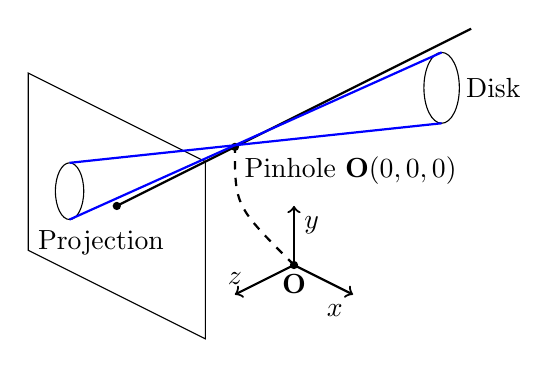
\begin{tikzpicture}[xscale=0.75, yscale=0.75]
				% Define coordinates
				\coordinate (O) at (0,0);
				\coordinate (P) at (6,3);
				\coordinate (I) at (2,1);
				\coordinate (F) at (-1.5,-0.75);
				
				% Image plane
				\draw (F) ++(0,0) -- ++(0,3) -- ++(3,-1.5) -- ++(0,-3) -- cycle;
				\fill (I) circle (2pt) node[below right] {Pinhole $\mathbf{O}(0,0,0)$};
				\fill (O) circle (2pt);
				
				\draw[thick] (O) -- (I);
				\draw[thick] (P) -- (I);
				
				\draw (F) ++(0.7,1) ellipse (0.3*0.8cm and 0.6*0.8cm);
				\draw (F) ++(0,0.5) node[below right] {Projection};
				\draw (P) ++(-0.5,-1) ellipse (0.3cm and 0.6cm);
				\draw (P) ++(-0.25, -1) node[right] {Disk};
				\draw[blue, thick] (P) ++(-0.5,-1+0.6) --  (-0.8, -0.75+1-0.48);
				\draw[blue, thick] (P) ++(-0.5,-1-0.6) --  (-0.8, -0.75+1+0.48);
				
				\coordinate (O1) at (3,-1);
				\coordinate (X) at (4,-1.5);
				\coordinate (Y) at (3,0);
				\coordinate (Z) at (2,-1.5);
				
				% Draw the axes
				\draw[->,thick] (O1) -- (X) node[anchor=north east]{$x$};
				\draw[->,thick] (O1) -- (Y) node[anchor=north west]{$y$};
				\draw[->,thick] (O1) -- (Z) node[anchor=south]{$z$};
				\draw[dashed,thick] (O1) .. controls (2,0) .. (I);
				
				% Draw the origin point
				\fill (O1) circle (2pt) node[below] {$\mathbf{O}$};
			\end{tikzpicture}		
		\caption{Disk before pinhole camera}	
		\label{1}
		\end{figure}
	
		\item The normal vector of the plane is $(A, B, C)^T$. Thus for the first case where $A=C=D=0, B=1$, the normal vector is $\mathbf{n} = (0, 1, 0)^T$. The plane, let's call it $\mathcal F_1$, is perpendicular to the y-axis at $y=0$, as shown in Figure \ref{2}. We represent a line with:
		\begin{equation}
			\begin{aligned}
				&\begin{cases}
					x = x_0 + t \cdot d_x \\
					y = y_0 + t \cdot d_y \\
					z = z_0 + t \cdot d_z
				\end{cases}, 
			&\text{or }\mathbf{x} = \mathbf{x_0} + t\mathbf{d}.
			\end{aligned}
		\end{equation}
		\begin{figure}[ht!]
			\centering
			\begin{minipage}{0.4\linewidth}
				\centering
				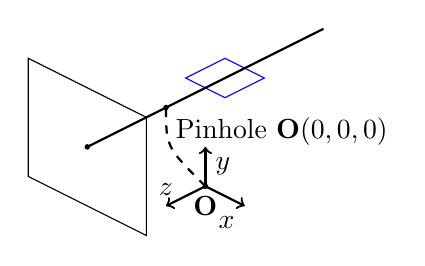
\begin{tikzpicture}[xscale=0.5, yscale=0.5]
					% Define coordinates
					\coordinate (O) at (0,0);
					\coordinate (P) at (6,3);
					\coordinate (I) at (2,1);
					\coordinate (F) at (-1.5,-0.75);
					\coordinate (W) at (3,1.5);
					
					\draw[blue] (W) ++(-0.5,0.25) -- ++(1,-0.5) -- ++(1,0.5) -- ++(-1,0.5) -- cycle;
					
					% Image plane
					\draw (F) ++(0,0) -- ++(0,3) -- ++(3,-1.5) -- ++(0,-3) -- cycle;
					\fill (I) circle (2pt) node[below right] {Pinhole $\mathbf{O}(0,0,0)$};
					\fill (O) circle (2pt);
					
					\draw[thick] (O) -- (I);
					\draw[thick] (P) -- (I);
					
					\coordinate (O1) at (3,-1);
					\coordinate (X) at (4,-1.5);
					\coordinate (Y) at (3,0);
					\coordinate (Z) at (2,-1.5);
					
					% Draw the axes
					\draw[->,thick] (O1) -- (X) node[anchor=north east]{$x$};
					\draw[->,thick] (O1) -- (Y) node[anchor=north west]{$y$};
					\draw[->,thick] (O1) -- (Z) node[anchor=south]{$z$};
					\draw[dashed,thick] (O1) .. controls (2,0) .. (I);
					
					% Draw the origin point
					\fill (O1) circle (2pt) node[below] {$\mathbf{O}$};
				\end{tikzpicture}
			
			\end{minipage}
			\hfill
			\begin{minipage}{0.4\linewidth}
				\centering
				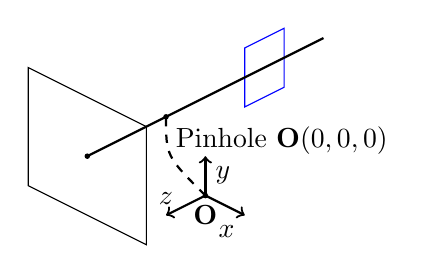
\begin{tikzpicture}[xscale=0.5, yscale=0.5]
					% Define coordinates
					\coordinate (O) at (0,0);
					\coordinate (P) at (6,3);
					\coordinate (I) at (2,1);
					\coordinate (F) at (-1.5,-0.75);
					\coordinate (W) at (3,1.5);
					
					\draw[blue] (W) ++(1,-0.25) -- ++(1,0.5) -- ++(0,1.5) -- ++(-1,-0.5) -- cycle;
					
					% Image plane
					\draw (F) ++(0,0) -- ++(0,3) -- ++(3,-1.5) -- ++(0,-3) -- cycle;
					\fill (I) circle (2pt) node[below right] {Pinhole $\mathbf{O}(0,0,0)$};
					\fill (O) circle (2pt);
					
					\draw[thick] (O) -- (I);
					\draw[thick] (P) -- (I);
					
					\coordinate (O1) at (3,-1);
					\coordinate (X) at (4,-1.5);
					\coordinate (Y) at (3,0);
					\coordinate (Z) at (2,-1.5);
					
					% Draw the axes
					\draw[->,thick] (O1) -- (X) node[anchor=north east]{$x$};
					\draw[->,thick] (O1) -- (Y) node[anchor=north west]{$y$};
					\draw[->,thick] (O1) -- (Z) node[anchor=south]{$z$};
					\draw[dashed,thick] (O1) .. controls (2,0) .. (I);
					
					% Draw the origin point
					\fill (O1) circle (2pt) node[below] {$\mathbf{O}$};
				\end{tikzpicture}
			\end{minipage}
			\caption{Vanishing point of planes}
			\label{2}
		\end{figure}
		For lines on $\mathcal F_1$, we have $\mathbf{d}\cdot\mathbf{n} = 0$, which means $d_y=0$ while $d_x$ and $d_z$ are arbitrary. In class we know the vanishing point of the line is $(f\frac{d_x}{d_z}, f\frac{d_y}{d_z})$. This shows the vanishing points are on line.
		\begin{equation}
			\begin{cases}
				y = 0 \\
				z = f
			\end{cases}.
		\end{equation}
	
		Therefore, for three given directions $(1,0,2)$, $(2,0,1)$ and $(1,0,1)$ on the plane, their vanishing point are $(\frac{f}{2}, 0)$, $(2f, 0)$, $(f, 0)$ respectively. 
		
		Similarly, for the second case, the vanishing points are on
		\begin{equation}
			\begin{cases}
				x = 0 \\
				z = f
			\end{cases}.
		\end{equation}
		For three given directions $(0,1,2)$, $(0,2,1)$ and $(0,1,1)$ on the plane, their vanishing point are $(0, \frac{f}{2})$, $(0, 2f)$, $(0, f)$ respectively. 
		\item In the last problem we have $\mathbf{d}\cdot\mathbf{n} = 0$, or $d_x\cdot A+d_y\cdot B+d_z\cdot C = 0$. We can further get
		\begin{equation}
			f\frac{d_x}{d_z}\cdot A+f\frac{d_y}{d_z}\cdot B+fC = 0,
		\end{equation}
		and this shows $x\cdot A+y\cdot B + f\cdot C = 0$ is the vanishing points of all lines on the given plane.
	\end{enumerate}
	\section*{Programming Assignment}
	\begin{enumerate}[1)]
		\item
		\begin{enumerate}[a.]
			\item To do this, since opencv returns a numpy array, simply use \texttt{np.where} to replace values higher than threshold with 255 else 0. It's silly to use if-else and scan instead. The choice of threshold is highly dependent to the image. Neither mean, medium nor diagram valleys would be proper. For given pictures, 128 works fine. 
			\item I use a union-find set to store labels. In my implementation, I scan from the bottom-left corner as clarified(in slides we start from top-left as default, however).
			
			I first initialize the first row of pixels. Then I scan the image with a $2\times2$ array $\left[\begin{matrix} A & B \\ C & D \end{matrix}\right]$. Before scanning each row, the first column pixel $A$ is initialized by $C$ and $D$. During scanning, we merge labels of $A$ and $D$ using union-find set and update $B$ if $B$ is not background. $B$ will be assigned the label of $A, C, D$(sequence do not matter) or a new label if $A, C, D$ are background. 
			
			In the end, I paint the labels with gray-scale color. To better visualize, I used a gamma transform function with parameter 2.2.
			\item I implement this function completely based on equations on slides. Nothing special here.
			
			The images are shown in Figure \ref{p1}. The first row are binary and the second are labeled. The output of three images are(the same sequence as images, kept the first two labels each with .2f):
			\begin{minted}{python}
{'position': {'x': 349.33, 'y': 215.45}, 'orientation': -1.26, 'roundness': 1.30}
{'position': {'x': 195.32, 'y': 222.38}, 'orientation': 0.69, 'roundness': 2.04}

{'position': {'x': 303.57, 'y': 177.27}, 'orientation': 0.41, 'roundness': 2.42}
{'position': {'x': 417.72, 'y': 240.29}, 'orientation': -0.78, 'roundness': 40.93}

{'position': {'x': 413.66, 'y': 203.95}, 'orientation': -1.12, 'roundness': 3.94}
{'position': {'x': 265.97, 'y': 168.65}, 'orientation': -0.49, 'roundness': 1.75}
			\end{minted}
			
			
			\begin{figure}[ht!]
				\centering
				\begin{minipage}{0.2\textwidth}
					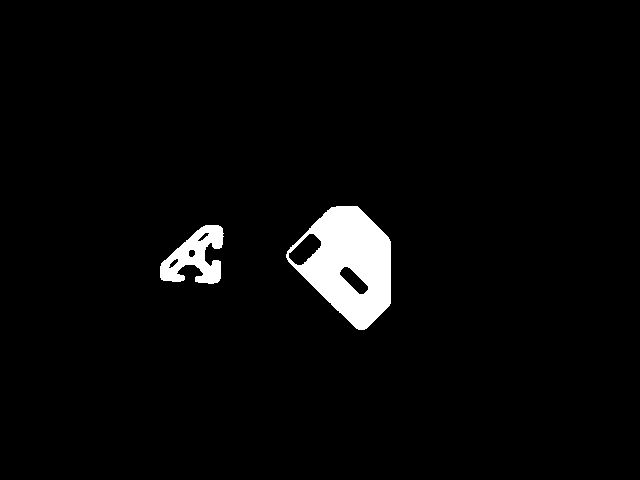
\includegraphics[width=\linewidth]{../output/two_objects_binary}
				\end{minipage}
			\hfill
				\begin{minipage}{0.2\textwidth}
					
\includegraphics[width=\linewidth]{../output/many_objects_1_binary}
				\end{minipage}
			\hfill
				\begin{minipage}{0.2\textwidth}
					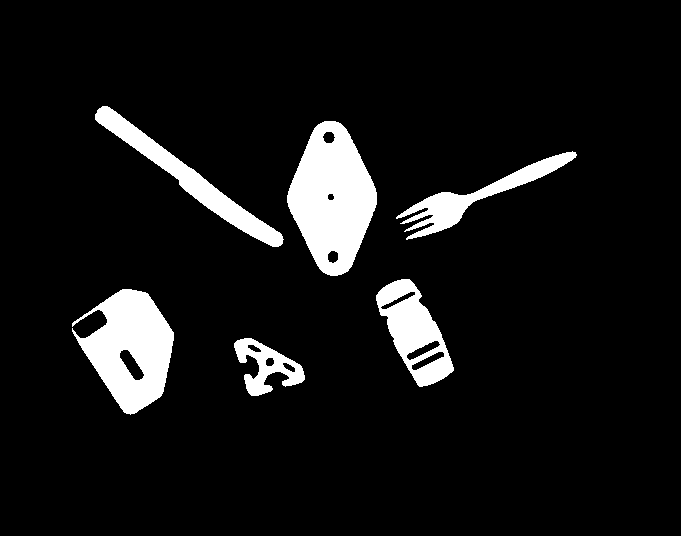
\includegraphics[width=\linewidth]{../output/many_objects_2_binary}
				\end{minipage}
				
				
				\begin{minipage}{0.2\textwidth}
					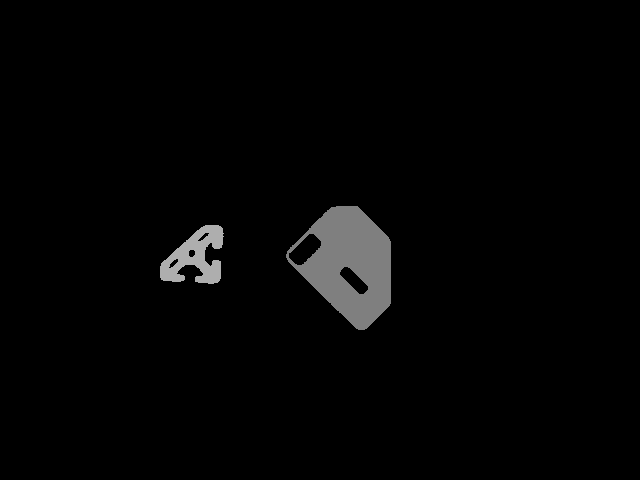
\includegraphics[width=\linewidth]{../output/two_objects_labeled}
				\end{minipage}
			\hfill
				\begin{minipage}{0.2\textwidth}
					
\includegraphics[width=\linewidth]{../output/many_objects_1_labeled}
				\end{minipage}
			\hfill
				\begin{minipage}{0.2\textwidth}
					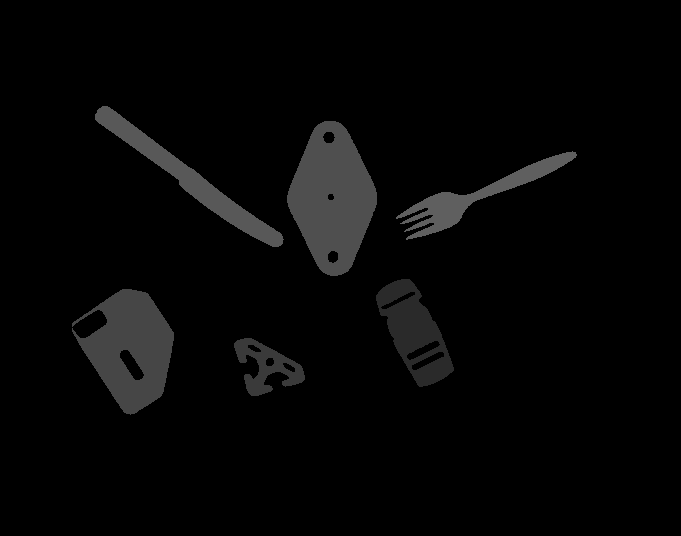
\includegraphics[width=\linewidth]{../output/many_objects_2_labeled}
				\end{minipage}
				\caption{Output Images}
				\label{p1}
			\end{figure}
		 
		\end{enumerate}
		\item
		\begin{enumerate}[a.]
			\item The given \texttt{coins.png} has obvious edges, and thus smaller Sobel operator(i.e. $3\times 3$) should work fine. To compare, I referred to the official doc of OpenCV. No significant difference is found. 
			\item I used \texttt{np.where} to finish the first task of this problem. For the second one, I considered traverse all the theta from 0 to 360 degree. At first I doubted it, for some pixels are counted multiple times. However, I get to know that people indeed do the same thing while rasterizing. In fact, multiple counts implies the pixel is closer to the round edge than others. 
			
			It really takes a second using merely \texttt{np}. I checked the array from problem 1. The maximum reaches 781, and thus I choose 350 as threshold. Since the circles are obvious enough, I did not further modify. Choices of radius are from 15 to 35. To calculate faster, I calculate the whole image as one for each theta. Furthermore,
			the coins do not look like standard circles, so I added ellipse correction.
			\item This function is only to find the local maximum and draw circles. Nothing is special. The threshold is to make every coin circled. Some coins are circled multiply times, and this is because they are not standard circles. Pick anyone of the output circle is fine. 
			
			The output are in Figure \ref{p2}. The program finishes within 2 seconds on an old CPU.
			
			\begin{figure}[ht!]
				\centering
				\begin{minipage}{0.2\textwidth}
					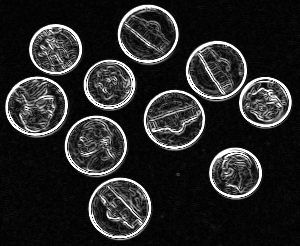
\includegraphics[width=\linewidth]{../output/coins_edge_raw}
					\caption{edge\_raw}
				\end{minipage}
			\hfill
				\begin{minipage}{0.2\textwidth}
					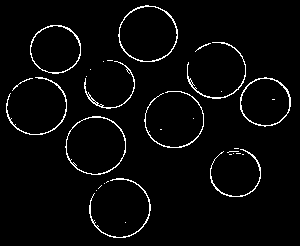
\includegraphics[width=\linewidth]{../output/coins_edge}
					\caption{coins\_edge}
				\end{minipage}
			\hfill
				\begin{minipage}{0.2\textwidth}
					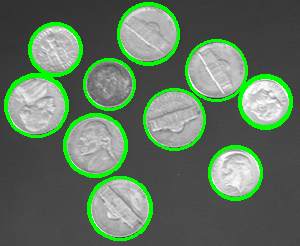
\includegraphics[width=\linewidth]{../output/coins_circle}
					\caption{coins\_circle}
				\end{minipage}
				
				\caption{Output Images 2}
				\label{p2}
			\end{figure}
			 
		\end{enumerate}
	\end{enumerate}
	\begin{figure}[h]
		\centering
		
\includegraphics[width=0.4\linewidth]{screenshot001}
	\end{figure}
	
\end{document}